\let\negmedspace\undefined
\let\negthickspace\undefined
\documentclass[journal]{IEEEtran}
\usepackage[a5paper, margin=10mm, onecolumn]{geometry}
%\usepackage{lmodern} % Ensure lmodern is loaded for pdflatex
\usepackage{tfrupee} % Include tfrupee package

\setlength{\headheight}{1cm} % Set the height of the header box
\setlength{\headsep}{0mm}     % Set the distance between the header box and the top of the text

\usepackage{gvv-book}
\usepackage{gvv}
\usepackage{cite}
\usepackage{amsmath,amssymb,amsfonts,amsthm}
\usepackage{algorithmic}
\usepackage{graphicx}
\usepackage{textcomp}
\usepackage{xcolor}
\usepackage{txfonts}
\usepackage{listings}
\usepackage{enumitem}
\usepackage{mathtools}
\usepackage{gensymb}
\usepackage{comment}
\usepackage[breaklinks=true]{hyperref}
\usepackage{tkz-euclide} 
\usepackage{listings}
% \usepackage{gvv}                                        
\def\inputGnumericTable{}                                 
\usepackage[latin1]{inputenc}                                
\usepackage{color}                                            
\usepackage{array}                                            
\usepackage{longtable}                                       
\usepackage{calc}                                             
\usepackage{multirow}                                         
\usepackage{hhline}                                           
\usepackage{ifthen}                                           
\usepackage{lscape}
\begin{document}

\bibliographystyle{IEEEtran}

\title{1.9.12}
\author{EE25BTECH11023 - Venkata Sai}
% \maketitle
% \newpage
% \bigskip
{\let\newpage\relax\maketitle}

\renewcommand{\thefigure}{\theenumi}
\renewcommand{\thetable}{\theenumi}

\numberwithin{equation}{enumi}
\numberwithin{figure}{enumi}
\renewcommand{\thetable}{\theenumi}

\textbf{Question}:\newline
Find the length of the segment joining \textbf{A}$\brak{-6,7}$ and \textbf{B}$\brak{-1,-5}$. Also, find the
midpoint of AB. 
\\
\textbf{Solution: }
\begin{table}[H]    
  \centering
  

  \caption{Variables Used}
\end{table}
Let the given points be
 \begin{align}
 \vec{A} = \myvec{-6 \\ 7}, \vec{B} = \myvec{-1 \\ -5} 
 \end{align}
The direction vector of the segment joining A and B is given by:
\begin{align}
\vec{B} - \vec{A} = \myvec{-1 - (-6) \\ -5 - 7} = \myvec{5 \\ -12} 
\end{align}
The length of the segment is the magnitude of the direction vector:
 \begin{align}
\vec{B} - \vec{A} = \myvec{-1 - (-6) \\ -5 - 7} = \myvec{5 \\ -12}  
\end{align}
\begin{align}
d = \|\vec{B-A}\| = \sqrt{\brak{B-A}^\top \brak{B-A}} 
\end{align}
\begin{align}
\brak{\vec{B}-\vec{A}}^\top \brak{\vec{B}-\vec{A}}&=\myvec{5  \ -12}\myvec{5 \\ -12}\\
&=5\times5+-12\times-12 = 169\\
d &=\sqrt{169}=13
\end{align}
Hence the length of the segment is 13 units. \\
To find midpoint of segment  $\vec{AB}$: \\
Let the required point be $\vec{P}$
\begin{align}
\vec{P}=\frac{k(\vec{B})+(\vec{A})}{k+1}
\end{align}
Here according to problem value of k is 1\\
\begin{align}
\vec{P}=\frac{\vec{B}+\vec{A}}{2}=\frac{\myvec{-6\\7}+\myvec{-1\\-5}}{2}=\frac{\myvec{-7\\2}}{2}\\
\end{align}
\begin{align}
\vec{P}=\myvec{\frac{-7}{2}\\1}
\end{align}
Hence the coordinates of $\vec{P}$ are $\brak{\frac{-7}{2},1}$
\begin{figure}[h!]
   \centering
   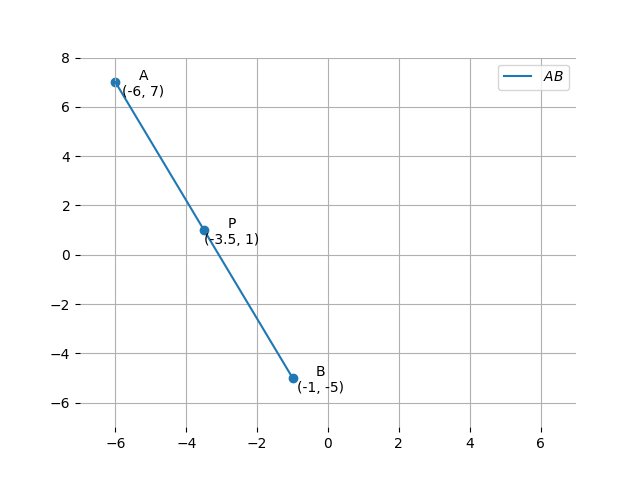
\includegraphics[width=0.7\columnwidth]{figs/fig1.png}
   \caption{Stem Plot of y\brak{n}}
   \label{stemplot}
\end{figure}
\end{document}  
